\documentclass[11pt,a4paper]{article}
\usepackage[margin=2.5cm]{geometry}
\usepackage{amsmath,amssymb,amsthm,tikz,pgfplots,xcolor,fancyvrb,hyperref,enumitem}
\pgfplotsset{compat=1.17}
\usepackage{fontspec}\setmonofont{DejaVu Sans Mono}[Scale=0.78]
\hypersetup{colorlinks=true,linkcolor=black,citecolor=blue!50!black,urlcolor=blue!50!black}
\newtheorem{theorem}{Slopollary}
\renewcommand{\thetheorem}{4}
\newtheorem{corollary}{Corollary}
\newtheorem{lemma}{Lemma}
\theoremstyle{definition}\newtheorem*{definition}{Definition}
\theoremstyle{remark}\newtheorem*{remark}{Remark}
\newcommand{\re}{\operatorname{Re}}
\newcommand{\C}{\mathbb{C}}\newcommand{\N}{\mathbb{N}}
\title{\textbf{Slopollary 4}\\[2pt]\large Which exponents does Li's criterion need?\\ Exactly a set of Bohr recurrence}
\author{Maths Slop}
\date{27 November 2026}
\begin{document}\maketitle

\begin{abstract}\noindent
Li's criterion tests whether points lie in the closed unit disc by checking that the sums
$\sum_j \re(1-\mu_j^n)$ are nonnegative for \emph{every} exponent $n\ge 1$; applied to the zeros of
$\zeta$ it is the Riemann hypothesis. We ask which sets $S$ of exponents are enough. For finite
families of points the answer is exact: the criterion works along $S$ if and only if $S$ is a set
of Bohr recurrence. So the multiples of a million are enough, while the primes are not: the single
point $2i$ passes every prime test. Everything is verified in Lean~4 with Mathlib.
\end{abstract}

\section{Statement}

For a finite family $\mu_1,\dots,\mu_k$ of complex numbers and $n\in\N$ write
\[ L_n(\mu)=\sum_{j=1}^{k}\re\bigl(1-\mu_j^{\,n}\bigr). \]
If every $|\mu_j|\le 1$ then $L_n(\mu)\ge 0$ for all $n$, trivially. The finite case of a theorem
of Bombieri and Lagarias~\cite{BL} is the converse: if $L_n(\mu)\ge 0$ for all $n\ge 1$ then every
$|\mu_j|\le1$. With $\mu=1-1/\rho$ over the zeros of $\zeta$ this is the mechanism behind Li's
criterion~\cite{Li} for the Riemann hypothesis.

\begin{definition}
Let $S\subseteq\N$.
\begin{itemize}[leftmargin=1.4em,itemsep=2pt]
\item \emph{Li's criterion works along $S$} if for every finite family $\mu$: whenever
$L_n(\mu)\ge0$ for all $n\in S$, every $|\mu_j|\le 1$.
\item $S$ is a \emph{set of Bohr recurrence} if for all $u_1,\dots,u_d$ on the unit circle and all
$\varepsilon>0$ there is $n\in S$, $n>0$, with $|u_j^{\,n}-1|<\varepsilon$ for every $j$. (Every
finite family of rotations returns close to the identity at a time in $S$.)
\end{itemize}
\end{definition}

\begin{theorem}
Li's criterion works along $S$ if and only if $S$ is a set of Bohr recurrence.
\end{theorem}

\begin{corollary}[enough]
For each $m\ge1$ the multiples of $m$ are a set of Bohr recurrence, so Li's criterion works along
them.
\end{corollary}

\begin{corollary}[not enough]
The primes are not a set of Bohr recurrence, so Li's criterion fails along the primes. Explicitly,
$\re\bigl(1-(2i)^p\bigr)\ge 0$ for every prime $p$, although $|2i|=2$.
\end{corollary}

\begin{corollary}[Riemann hypothesis along $S$]
Let $S$ be a set of Bohr recurrence. The Riemann hypothesis holds if and only if for every finite
set $Z$ of nontrivial zeros of $\zeta$ and every $n\in S$,
\[ \sum_{\rho\in Z}\re\Bigl(1-\bigl(1-\tfrac1\rho\bigr)^{n}\Bigr)\ \ge\ 0 . \]
\end{corollary}

\section{Proof}

\paragraph{Recurrence implies the criterion.}
Let $S$ be a set of Bohr recurrence and suppose some $|\mu_1|=r>1$. Write $\mu_j=|\mu_j|\,w_j$
with $|w_j|=1$ and pick $N$ with $r^N>2k$. Add one more rotation $v=e^{i}$, by one radian. Since
$\pi$ is irrational, $v^n\ne1$ for all $n\ge1$, so $\delta=\min_{1\le n\le N}|v^n-1|>0$. Recurrence
gives $n\in S$ with $|v^n-1|<\delta$ and all $|w_j^{\,n}-1|<\tfrac12$. The first forces $n>N$. The
second gives $\re w_j^{\,n}>\tfrac12$, hence $\re\mu_j^{\,n}\ge\tfrac12|\mu_j|^n\ge0$ for every
$j$, and
\[ L_n(\mu)\ \le\ k-\tfrac12 r^{n}\ \le\ k-\tfrac12 r^{N}\ <\ 0 . \]
So a point outside the disc is detected by an exponent in $S$.

\paragraph{The criterion implies recurrence.}
Suppose $S$ is not a set of Bohr recurrence: there are $u_1,\dots,u_d$ on the unit circle and
$0<\varepsilon\le1$ such that every positive $n\in S$ has some $j$ with
$|u_j^{\,n}-1|\ge\varepsilon$. (If $d=0$ then $S$ has no positive element and the single point
$\mu=2$ already beats the criterion.) We build finitely many points of modulus $2$ with
$L_n\ge0$ for all $n\in S$.

For $|z|=1$ we have $z\bar z=1$, so
\[ (1+z)^{2M}\,\bar z^{\,M}=\bigl((1+z)^2\bar z\bigr)^M=(2+2\re z)^M=\bigl(4-|z-1|^2\bigr)^M ,\]
and by the binomial theorem the left side is $\sum_{e=0}^{2M}\binom{2M}{e}z^{\,e-M}$. Multiplying
over $j$,
\begin{equation}\label{kernel}
\sum_{e\in\{0,\dots,2M\}^d} m(e)\,\chi_e(z)=\prod_{j=1}^{d}\bigl(4-|z_j-1|^2\bigr)^M,
\qquad m(e)=\prod_j\binom{2M}{e_j},\quad \chi_e(z)=\prod_j z_j^{\,e_j-M}.
\end{equation}
This is de la Vall\'ee-Poussin's kernel in $d$ variables. Its constant term is the frequency
$c=(M,\dots,M)$, with $\chi_c\equiv1$ and $m(c)=\binom{2M}{M}^d$.

\emph{The family:} for each $e\ne c$ take the point $2\chi_e(u)$, repeated $m(e)$ times. There are
$k=4^{Md}-\binom{2M}{M}^d>0$ points, all of modulus $2$. Since $\chi_e(u)^n=\chi_e(u^n)$,
identity \eqref{kernel} at $z=u^n$ gives
\[ L_n=k-2^n\Bigl(\prod_{j}\bigl(4-|u_j^{\,n}-1|^2\bigr)^M-\tbinom{2M}{M}^d\Bigr). \]
For positive $n\in S$ one factor is at most $(4-\varepsilon^2)^M$ and the others at most $4^M$, so
with $q=1-\varepsilon^2/4<1$ and the classical bound $4^M\le(2M+1)\binom{2M}{M}$,
\[ \prod_{j}\bigl(4-|u_j^{\,n}-1|^2\bigr)^M\le 4^{Md}q^M\le\tbinom{2M}{M}^d\,(2M+1)^d q^M
\le\tbinom{2M}{M}^d \]
once $M$ is large enough that $(2M+1)^dq^M\le1$. Then $L_n\ge k\ge0$ for every positive $n\in S$
(and $L_0=0$), while every point has modulus $2$. So the criterion fails along $S$. \qed

\begin{figure}[h]\centering
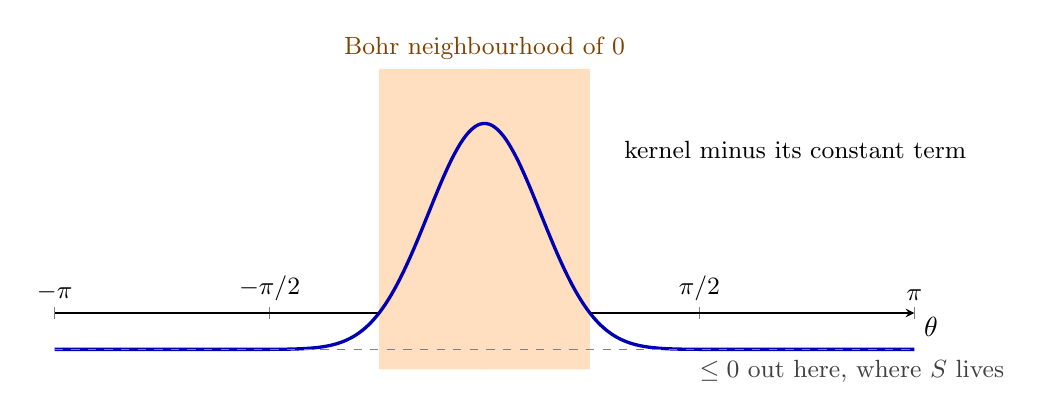
\begin{tikzpicture}
\begin{axis}[width=12.5cm,height=5.4cm,xmin=-3.1416,xmax=3.1416,ymin=-0.25,ymax=1.08,
  axis lines=middle,xtick={-3.1416,-1.5708,0,1.5708,3.1416},
  xticklabels={$-\pi$,$-\pi/2$,$0$,$\pi/2$,$\pi$},ytick={0.5,1},
  xlabel={$\theta$},x label style={at={(axis description cs:1.0,0.14)},anchor=west},
  tick label style={font=\small},xticklabel style={anchor=south,yshift=3pt},clip=false]
\addplot[fill=orange!25,draw=none] coordinates {(-0.770,-0.25) (0.770,-0.25) (0.770,1.08) (-0.770,1.08)} \closedcycle;
\addplot[domain=-3.1416:3.1416,samples=300,very thick,blue!70!black] {((1+cos(deg(x)))/2)^12-0.1612};
\addplot[domain=-3.1416:3.1416,samples=2,dashed,gray] {-0.1612};
\node[font=\small,anchor=west] at (axis cs:0.95,0.72) {kernel minus its constant term};
\node[font=\small,anchor=south,orange!50!black] at (axis cs:0,1.08) {Bohr neighbourhood of $0$};
\node[font=\small,anchor=north west,gray!50!black] at (axis cs:1.5,-0.165) {$\le 0$ out here, where $S$ lives};
\end{axis}
\end{tikzpicture}
\caption{One rotation, $M=12$: the function $\bigl(\tfrac{1+\cos\theta}{2}\bigr)^{12}-\binom{24}{12}4^{-12}$.
All its Fourier coefficients are $\ge0$ and it has no constant term, yet it is $\le 0$ outside a
neighbourhood of $0$. If the angles $n\theta$, $n\in S$, avoid that neighbourhood, the points
built from its frequencies fool Li's criterion along $S$.}
\end{figure}

\section{Examples}
\begin{itemize}[leftmargin=1.4em,itemsep=3pt]
\item \textbf{All $n\ge1$.} Compactness of the torus gives recurrence, and the theorem returns the
finite Bombieri--Lagarias criterion (Slopollary~3).
\item \textbf{Multiples of $m$.} Apply the previous case to the rotations $u_j^{\,m}$.
\item \textbf{Primes.} The quarter turn $u=i$ never returns: $i^p\in\{-1,i,-i\}$ for prime $p$, so
$|i^p-1|\ge1$. A witness needs no kernel: $(2i)^2=-4$ and $(2i)^p=\pm2^p i$ for odd $p$, so the
Li test of the single point $2i$ gives $5$ at $p=2$ and $1$ at every odd prime.
\item \textbf{Odd numbers.} The pair $\{2,-2\}$ has $L_n=2$ for every odd $n$. (By hand; not in
the Lean file.)
\item \textbf{Not formalised, quoted from the literature.} Lacunary sets such as $\{2^k\}$ and
$\{k!\}$ are not sets of Bohr recurrence~\cite{lac}, so the criterion fails along them, even though
every integer divides some factorial. The squares are a set of recurrence
(Furstenberg, S\'ark\"ozy), hence of Bohr recurrence, so the criterion works along $n=k^2$.
\end{itemize}

\section{What is new and what is not}
\begin{itemize}[leftmargin=1.4em,itemsep=3pt]
\item \emph{Not ours.} Li's criterion~\cite{Li}; the Bombieri--Lagarias theorem~\cite{BL}; sets of
Bohr recurrence, a standard notion in additive combinatorics and dynamics; the
de la Vall\'ee-Poussin kernel. Power sums over a prescribed set of exponents, including one-sided
problems, are the subject of Tur\'an's power sum method~\cite{Turan}; a specialist there may well
know this statement.
\item \emph{What we could not find.} The equivalence ``Li's criterion along $S$ $\Leftrightarrow$
$S$ is a set of Bohr recurrence'', the failure along the primes, or any Lean formalisation of
either. We searched for Li's criterion along subsequences and arithmetic progressions, for
Bombieri--Lagarias together with Bohr recurrence, and for one-sided power sum problems together
with Bohr recurrence. The searches were short; if you know a source, open an issue and we will
credit it.
\item \emph{Limits.} The theorem is about arbitrary finite families of points. It does not say that
the genuine Li coefficients $\lambda_n$ (infinite sums over all zeros) fail to characterise the
Riemann hypothesis along the primes; zeros of $\zeta$ are not arbitrary points. The last corollary
is an equivalence of statements, proved without using the Riemann hypothesis; since the hypothesis
is now a theorem (Alp\"oge, 20 November 2026), both sides are true.
\item \emph{Depth.} A real two-sided proof, at the level of a first course in harmonic analysis:
compactness one way, a positive kernel the other. Not deep.
\end{itemize}

\section{Formalisation}
The file \texttt{Slopollary4.lean} (741 lines) compiled on \url{https://live.lean-lang.org}
(Lean 4.37.0-rc1, latest Mathlib) on 27 November 2026, exactly as published, with no errors, no
warnings and no \texttt{sorry}. For each theorem below \texttt{\#print axioms} reported
\texttt{[propext, Classical.choice, Quot.sound]}. The Riemann hypothesis is not imported; it
appears only as Mathlib's statement \texttt{RiemannHypothesis} inside the last equivalence.

\begin{Verbatim}[frame=single,rulecolor=\color{gray!50},fontsize=\small]
def BohrRecurrent (S : Set ℕ) : Prop :=
  ∀ (κ : Type) [Fintype κ] (u : κ → ℂ), (∀ j, ‖u j‖ = 1) → ∀ ε : ℝ, 0 < ε →
    ∃ n ∈ S, 0 < n ∧ ∀ j, ‖u j ^ n - 1‖ < ε

def LiAlong (S : Set ℕ) : Prop :=
  ∀ (ι : Type) [Fintype ι] (μ : ι → ℂ),
    (∀ n ∈ S, 0 ≤ ∑ j, (1 - μ j ^ n).re) → ∀ j, ‖μ j‖ ≤ 1

theorem liAlong_iff_bohrRecurrent (S : Set ℕ) : LiAlong S ↔ BohrRecurrent S

theorem liAlong_multiples {m : ℕ} (hm : 0 < m) : LiAlong {n : ℕ | m ∣ n}

theorem not_liAlong_primes : ¬LiAlong {p : ℕ | p.Prime}

theorem two_I_passes_prime_tests {p : ℕ} (hp : p.Prime) :
    0 ≤ (1 - (2 * Complex.I) ^ p).re

theorem riemannHypothesis_iff_finite_li_sums_along {S : Set ℕ} (hS : BohrRecurrent S) :
    RiemannHypothesis ↔
      ∀ Z : Finset ℂ, (∀ ρ ∈ Z, IsNontrivialZero ρ) →
        ∀ n ∈ S, 0 ≤ ∑ ρ ∈ Z, (1 - (1 - 1 / ρ) ^ n).re
\end{Verbatim}
The human proof above and the Lean proof follow the same steps: \texttt{exists\_neg\_li\_sum\_along}
is the first paragraph (with \texttt{exp\_I\_pow\_ne\_one} for the irrational rotation), and
\texttt{sum\_mult\_phase}, \texttt{kernel\_le} and \texttt{not\_liAlong\_aux} are the kernel
identity, the kernel bound and the family. Full source and this paper:
\url{https://github.com/slopollary/slopollaries/tree/main/04-recurrence}.

\begin{thebibliography}{9}\small
\bibitem{Li} X.-J. Li, The positivity of a sequence of numbers and the Riemann hypothesis,
\emph{J. Number Theory} 65 (1997), 325--333.
\bibitem{BL} E. Bombieri and J. C. Lagarias, Complements to Li's criterion for the Riemann
hypothesis, \emph{J. Number Theory} 77 (1999), 274--287.
\bibitem{Turan} P. Tur\'an, \emph{On a New Method of Analysis and its Applications}, Wiley, 1984.
\bibitem{lac} \emph{Bohr recurrence and density of non-lacunary semigroups of $\N$},
arXiv:2406.01353; the introduction recalls that no lacunary set is a set of Bohr recurrence.
\end{thebibliography}
\end{document}
